\chapter{Manual de la Aplicacion}
% ------------------------------------------------------------------------------
\section{Conexión USB}
Como se menciono en las secciones anteriores, se requiere el adaptador RS232-USB, por tal motivo se adjunta el driver correspondiente a el modelo utilizado en el Laboratorio.

Al abrir la aplicación se tiene la sección de \textbf{Conexión}, Después de seleccionar el puerto COM y la Velocidad de Transmisión correspondiente al Osciloscopio, si se presiona \textbf{Conectar} se visualizara el siguiente mensaje.


\begin{center}
	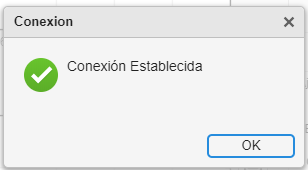
\includegraphics[width=0.3\columnwidth]{images/Conexion_Ok}
	\captionsetup{type=figure}
	\caption{Cuadro de dialogo - Conexión Exitosa}
	\label{fig:002}
\end{center}

En este momento, el bus de datos no se encuentra ocupado, simplemente configuro el Encoding y luego verifico el modelo del osciloscopio. Ahora se permite leer los valores del osciloscopio.

Al presionar \textbf{Leer Valores} realizara la rutina desarrollada en la sección anterior. Lee los parámetros correspondiente al tiempo, luego el canal 1 junto con sus parámetros y por ultimo el canal 2 con sus parámetros. Finalmente, la aplicación armara el vector de tensión, y con la cantidad de puntos leídos estará en condiciones de armar el vector de tiempo.

En caso de existir algún error en la comunicación o en los datos, se visualizara en pantalla con un mensaje indicando el mismo.


\begin{center}
	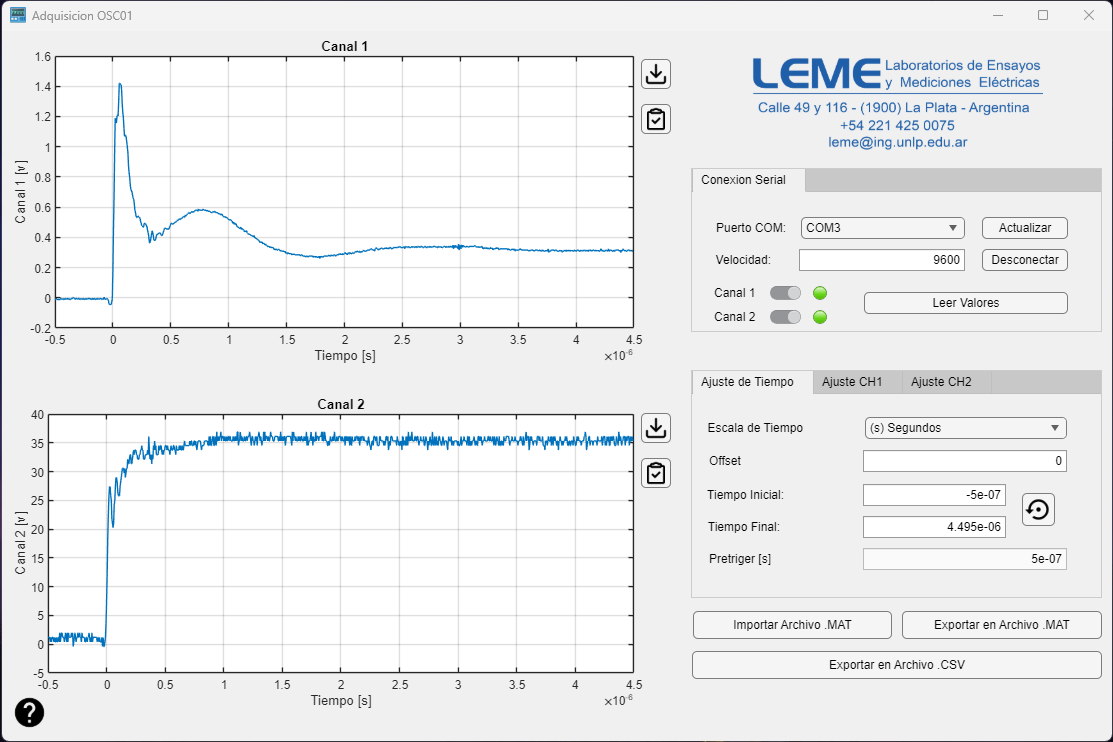
\includegraphics[width=0.7\columnwidth]{images/Datos_Leidos}
	\captionsetup{type=figure}
	\caption{Descarga correcta de valores}
	\label{fig:003}
\end{center}

Una vez leído los valores y presentados en los ejes correspondientes, se habilitan los controles correspondiente al tiempo, y a los volts en cada canal.



\subsection{Ajustes de Tiempo}
La sección de Ajustes de Tiempo permite cambiar las unidades de la escala de tiempo, de esta forma se elimina el multiplicador $x10^{-6}$ como se ve en la imagen \ref{fig:003}.

\begin{center}
	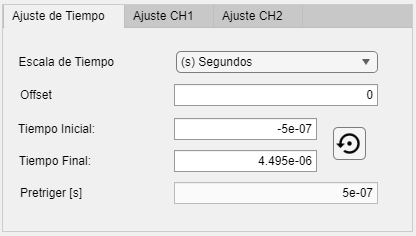
\includegraphics[width=0.4\columnwidth]{images/Ajuste_Tiempo}
	\captionsetup{type=figure}
	\caption{Control de ajustes de tiempo}
	\label{fig:004}
\end{center}

Ademas, se permite configurar un Offset de tiempo, en las unidades elegidas en el selector. Esto permite desplazar el valor de tiempo cero con el fin de anular el tiempo del pre-triger, o bien simplemente desplazar el eje de tiempo.

Los dos campos de \textbf{Tiempo Inicial} y \textbf{Tiempo Final} permiten acotar la ventana de tiempo, con el fin de poder dejar visible una ventana de tiempo especifica. En caso de requerir restaurar la ventana al tiempo que muestreo el osciloscopio, se utiliza el boton para restablecerlo, ubicado entre los dos campos nombrados.

Finalemente, el ultimo campo no es editable y simplemente deja visualizar el valor de tiempo que dura el pre-triger, es decir, sera el tiempo transcurrido entre la primer muestra y el disparo del triger.


\subsection{Ajustes de los Canales}

Al igual que los ajustes de tiempo, se permite ajustar algunos parámetros de las gráficas de cada canal. Los primeros dos, \textbf{Titulo} y \textbf{Etiqueta} son los textos que aparecerán en las gráficas, siendo esto de ayuda para el momento en que se deba exportar la imagen para algún informe.

\begin{center}
	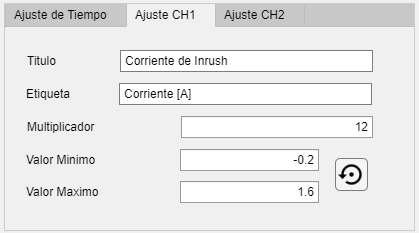
\includegraphics[width=0.4\columnwidth]{images/Ajuste_Canal1}
	\captionsetup{type=figure}
	\caption{Control de ajustes de tiempo}
	\label{fig:005}
\end{center}

El \textbf{Multiplicador} permitirá aplicar un factor por el cual se multiplica cada elemento del vector de tensión correspondiente al canal de la ficha seleccionada.

Los valores de \textbf{Valor Mínimo} y \textbf{Valor Máximo} simplemente ajustan los limites del eje vertical con el fin de dar libertad al momento de exportar la imagen. También se dispone del botón que permite restablecer y ajustar los limites a la amplitud de la curva.

En el Canal 2, se dispone de los mismos parámetros, siendo aplicados a la grafica inferior.

\section{Exportar en Archivo .MAT} \label{Exportar en Archivo .MAT}

El archivo \code{.mat} es propio de MatLab y permite que desde el propio software se puedan leer las variables para lograr manipular o trabajar con estas muestras leídas.

Para generar este archivo, simplemente se presiona el botón \textbf{Exportar en Archivo .MAT}. Se abrira una ventana donde se ubicara seleccionara la ruta y el nombre del mismo, logrando así generar el archivo en cuestión.

Para no modificar la información que se leyó, se devuelve la siguiente estrura de datos:

\begin{itemize}
	\item \code{dt}: Es el valor de tiempo entre muestras.
	\item \code{offset_t}: Es el desplazamiento que se realiza por el usuario en el vector tiempo.
	\item \code{ch1}: Contiene los datos del canal 1, los cuales seran:
	\begin{itemize}
		\item \code{ch1.raw}: Sera el vector que contiene la totalidad de las muestras leidas, correspondientes al canal 1.
		\item \code{ch1.ymult}: Es el factor por el cual se debera multiplicar cada muestra.
		\item \code{ch1.yoff}: Es el valor que se le debera restar al valor RAW leido (antes de usar el multiplicador).
		\item \code{ch1.yzero}: Es el valor de tensión que se le deberá sumar al valor ya convertido en tensión.
		\item \code{ch1.titulo}: Corresponde al texto usado en el titulo de la gráfica.
		\item \code{ch1.leyenda}: Corresponde al texto usado en la leyenda del eje vertical.
	\end{itemize}
	\item \code{ch2}: Se repite la misma estructura que en \code{ch1}.
\end{itemize}

Para lograr usar estos valores en matlab, se puede implementar el siguiente script:

\begin{lstlisting}[style=Matlab, firstnumber=1]
	load('NombreArchivo.MAT');
	
	t = (0:dt:(length(ch1.raw) - 1)*dt) - trig_pos;
	ch1_v = (ch1.raw - ch1.yoff) .* ch1.ymult + ch1.yzero;
	
	plot(t, ch1 .* ch1.factor)
\end{lstlisting}

De esta forma, en MatLab tendremos ahora el vector \code{t} y el vector \code{ch1_v}, los cuales representan el tiempo y los volts (del canal 1). El valor del factor que se utilizo como multiplicador se almacena en \code{ch1.factor}.



\section{Exportar como .CSV}

Para permitir exportar archivos y manipularlos en aplicaciones como Microsoft Excel, se implementa un botón que permite exportarlos con la extensión .CSV. Básicamente hace uso de la funcion \code{writetable()} de MatLab, la cual esta configurada para que guarde unicamente 3 columnas:

\begin{itemize}
	\item \code{Tiempo}: Es el valor del tiempo para cada muestra descargada.
	\item \code{CH1}: Serán las muestras, en Volts del canal 1.
	\item \code{CH2}: Al igual que el anterior, serán las muestras, en Volts del canal 2.
\end{itemize}

Por ultimo, el delimitador se configuro en \textbf{tabs}.


\section{Importar archivo .MAT}
La importación de estos archivo permite que vuelva a visualizar la curva que se encontraba almacenada en el archivo .MAT, de esta forma se podria modificar los valores de los campos disponibles y volver a guardar en un archivo nuevo, o bien como alternativa para editar y luego sobrescribir el archivo.

Para esto, la aplicación dispone del botón \textbf{Importar Archivo .MAT}, la cual primero verificara que las variables mencionadas en la sección \ref{Exportar en Archivo .MAT} estén todas contenidas en el archivo. Si se cumple esta condición, entonces se cargaran los vectores y los valores, completando así en cada campo el valor correspondiente.






\section{Exportar Imágenes}
Para esta funcionalidad, se dispone de dos métodos:

\begin{center}
	
\includegraphics[width=0.06\columnwidth]{images/Boton_ExportImage}
	\captionsetup{type=figure}
	\caption{Botones para exportar imagen}
	\label{fig:006}
\end{center}

El primero corresponde permite \textbf{Descargar} como un archivo de imagen, mientras que el segundo permite \textbf{Copiar} al portapapeles. Como se vera a continuación, cada uno de ellos permitirá elegir la extensión de la imagen.



\subsection{Exportar como Archivo de Imagen}
Al presionar el primer botón, aparecerá un cuadro de dialogo que permitirá seleccionar si el archivo se exportara como imagen vectorial (PDF), o simplemente como una imagen (PNG).
\begin{center}
	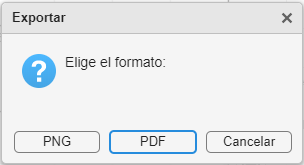
\includegraphics[width=0.4\columnwidth]{images/Export_ImageFile}
	\captionsetup{type=figure}
	\caption{Selección del Formato}
	\label{fig:007}
\end{center}

Luego de la selección, se solicitara la ruta y el nombre del archivo que se exportara.


\subsection{Exportar al Portapales}
Al presionar el segundo botón, aparecerá un cuadro de dialogo que permitira seleccionar si el archivo se copiara como imagen vectorial (SVG), o como simplemente imagen (PNG).

\begin{center}
	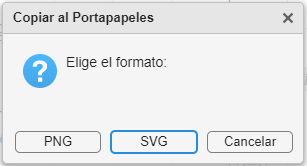
\includegraphics[width=0.4\columnwidth]{images/Export_Clipboard}
	\captionsetup{type=figure}
	\caption{Selección del Formato}
	\label{fig:008}
\end{center}

Luego de la selección, simplemente usar la imagen como si de un texto copiado se tratase.

























